\section{Test SPI Commands and Data Flow from Master Arduino to LTC6802 Chip}
This section provides the steps needed to use the slave-side simulation in SPI communication between Arduino chips. This is mainly written to be able to test the commands and data flow from the master Arduino board to the LTC6802 chip. This simulation simply prints out any data received from the master so that one can check the communication errors and debug them.

\subsection{User Manual}\label{sec:userMan}
\subsection{Step (1): Downloading Code and Setting up Your PC.}
Clone or download the IMHOTEP repository from the following link:\\
\url{https://github.com/mnourgwad/imhotep}
\begin{figure}[h]
\centering
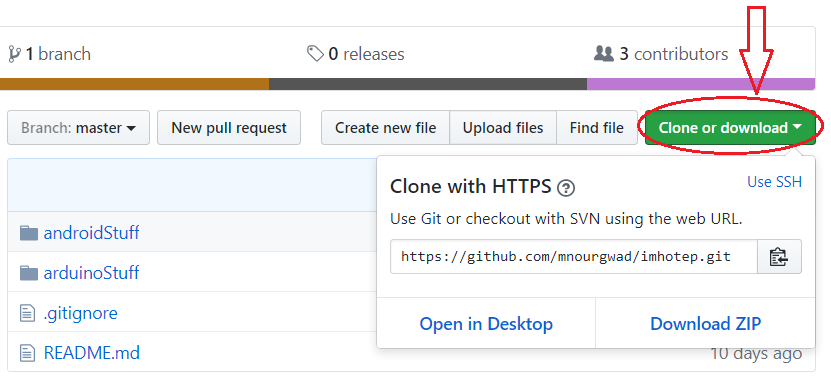
\includegraphics[width=13.82cm,height=6.33cm]{figures/image6}
\caption{Clone or download the IMHOTEP repository}
\end{figure}

\subsection{Step (2): Reaching the code.}
Now you have \texttt{imhotep} folder on your PC. It contains two main subfolders: \texttt{androidStaff}
 and \texttt{arduinoStaff} (see Fig.\ref{fig:projectfolders}). In this tutorial we work on the Arduino side.
\begin{figure}[h]
    \centering
    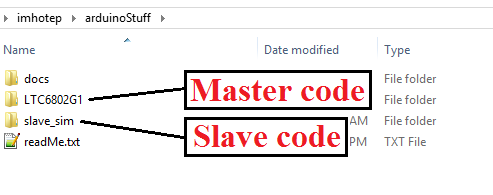
\includegraphics[width=11.55cm,height=4.56cm]{figures/image7}
    \caption{\texttt{imhotep} folder with code in the two subfolders}
    \label{fig:projectfolders}
\end{figure}

In \texttt{arduinoStaff} subfolder we have two Arduino projects:
\begin{enumerate}
\item \texttt{LTC6802G1}: This implements the master side.
\item \texttt{slave-sim}: This implements a slave-side in the SPI communication to simulate the IC operation and test the proper instruction and data flow controlled by the master side.
\end{enumerate}

\subsection{Step (3): Running the master-side.}
\begin{enumerate}
    \item Open \texttt{LTC6802G1} folder (see Fig.\ref{fig:LTC6802G1folders}).
    \item Open\texttt{LTC6802G1.ino} file. It will open in the Arduino IDE by default.
        \begin{figure}[h]
        \centering
        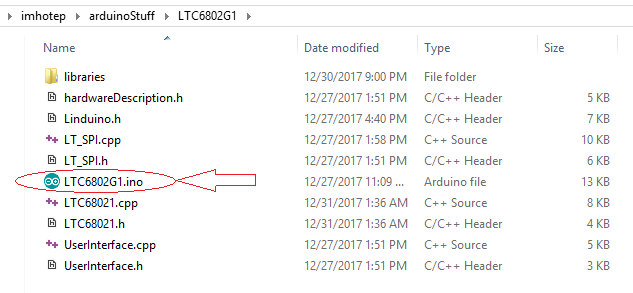
\includegraphics[width=13.90cm,height=6.44cm]{figures/image8}
        \caption{ \texttt{LTC6802G1} folder contents and \texttt{LTC6802G1.ino} file.}
            \label{fig:LTC6802G1folders}
        \end{figure}
\item Connect your Arduino board 'Master' to any serial port of your computer. 
Make sure that you selected the right Arduino board and serial port. In our 
tutorial we use Arduino Nano. Figure.\ref{fig:ArdConnection} shows the configuration we had (note that yours can be a bit different).
    \begin{figure}[h]
    \centering
    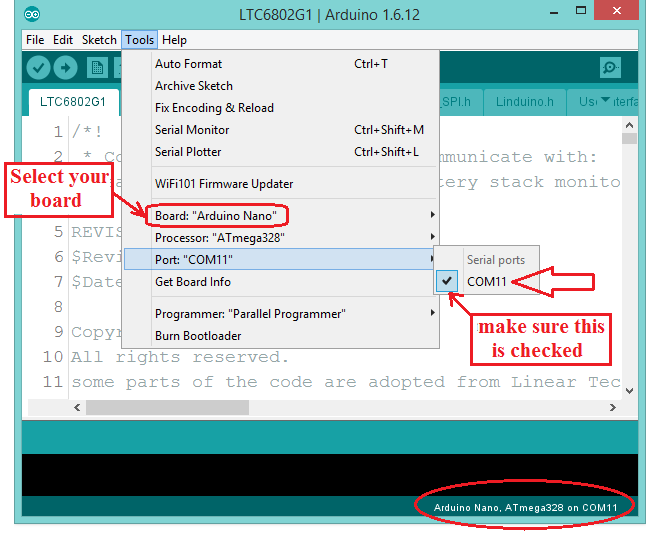
\includegraphics[width=11.21cm,height=9.19cm]{figures/image9}
    \caption{Arduino board connected to PC through USB port}
    \label{fig:ArdConnection}
    \end{figure}
\item Now we can upload the code on our board by clicking the 'upload' icon on 
the top-left corner of the Arduino window as shown in Fig.\ref{fig:Ardcodeupload}. 
    \begin{figure}[h]
        \centering
        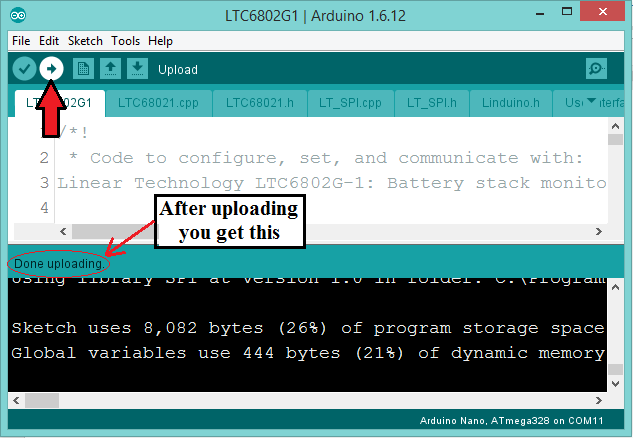
\includegraphics[width=11.11cm,height=7.69cm]{figures/image10}
        \caption{Uploading code to Arduino board.}
        \label{fig:Ardcodeupload}
    \end{figure}
\end{enumerate}

\subsection{Step (4): Running the salve-side.}
\begin{enumerate}
\item Open \texttt{slave\_sim} folder (see Fig.\ref{fig:slaveFolder}).
\item Double click on \texttt{slave\_sim.ino} file. It will open in the Arduino IDE by default.
    \begin{figure}[h]
        \centering
        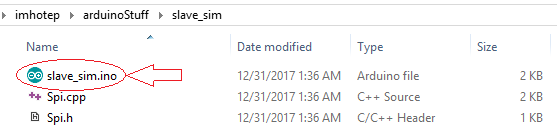
\includegraphics[width=12.75cm,height=3.08cm]{figures/image11}
        \caption{ \texttt{slave\_sim} folder contents and \texttt{slave\_sim.ino} file.}
                \label{fig:slaveFolder}
    \end{figure}
\item Connect your Arduino unit 'Master' to any serial port of your computer. 
Make sure that you selected the right Arduino board and serial port. In our 
tutorial we use Arduino Nano as in Fig.\ref{fig:ArdConnection}.
      \begin{figure}[h]
        \centering
        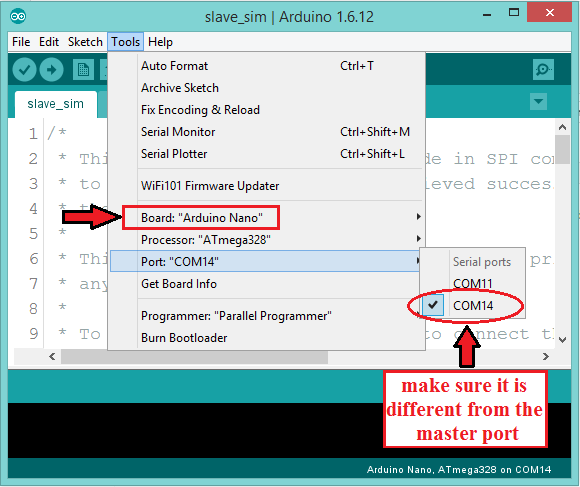
\includegraphics[width=11.21cm,height=9.19cm]{figures/image12}
        \caption{Arduino Master board connected to PC through USB port}
        \label{fig:ArdMasterConnection}
    \end{figure}
\item Click on the upload icon to upload the code on the slave board.
\end{enumerate}


\subsection{Step (5): Connecting slave to master (Hardware wiring).}
In Serial Peripheral Interface (SPI) communication there are four pins to connect. Table.\ref{tbl:ArdMasterConnection} describes these pins and their numbers in Arduino \textbf{Nano} board.
\begin{table}[h]
    \caption{Connecting slave to master (Hardware wiring).}
    \centering
\begin{tabular}{|l|l|l|}  \hline 
    1.  & Slave Select (SS) &  pin 10\\ \hline 
    2. & Master Out Slave In (MOSI) &  pin 11\\  \hline 
    3. & Master In Slave Out (MISO) & pin 12 \\  \hline 
    4.&  Serial clock (SCK)&  pin 13\\   \hline 
\end{tabular} 
        \label{tbl:ArdMasterConnection}
\end{table}

Connect each pin in master with the same pin in slave. Your circuit must be something like the one depicted in Fig.\ref{tbl:wiring}.
\begin{figure}[H]
\centering
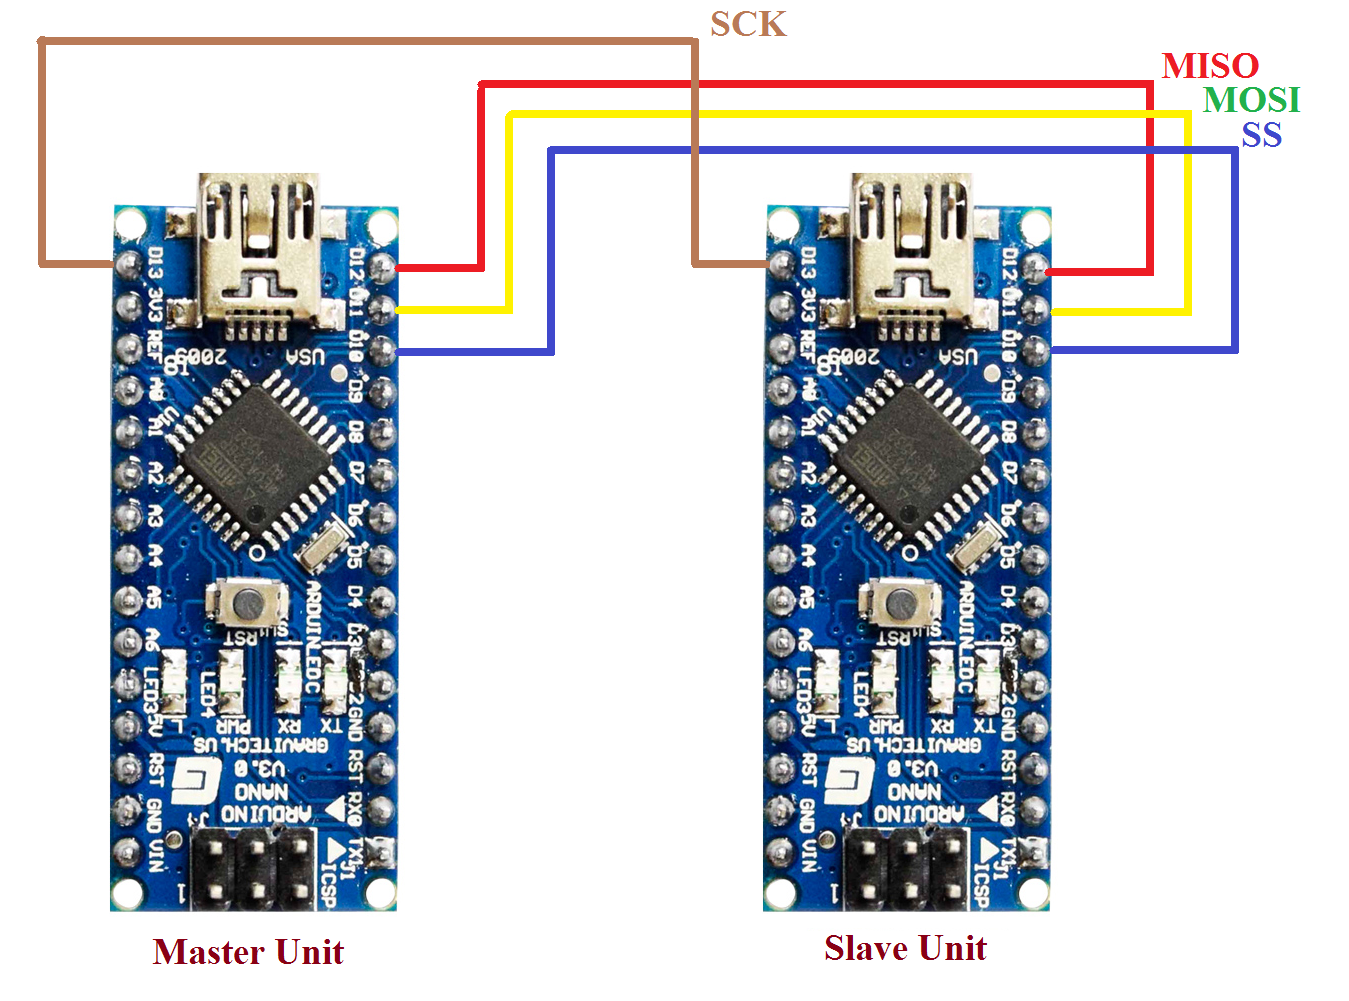
\includegraphics[width=0.6\textwidth]{figures/image13}
    \caption{Connecting slave to master (Hardware wiring).}
            \label{tbl:wiring}
\end{figure}

\subsection{Step (6): Running the Serial Monitor.}
There are two ways to open the serial monitor in Arduino IDE:
\begin{enumerate}
\item Click the icon in the top right corner.
\item From 'Tools' choose 'Serial Monitor' option (check Fig.\ref{fig:erialMon}).
\begin{figure}[h]
    \centering
    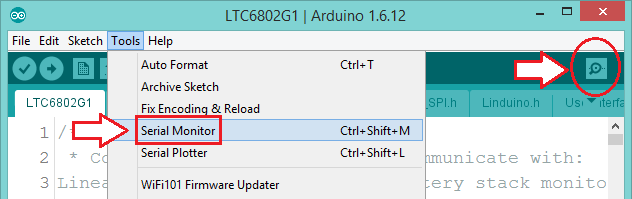
\includegraphics[width=10.38cm,height=3.27cm]{figures/image14}
    \caption{Running the serial monitor}
    \label{fig:erialMon}
\end{figure}
\end{enumerate}

Open the serial monitor in both master and slave Arduino windows. Make sure that the selected baud rate in the bottom right corner in the serial monitor is 115200 as it was initialized in the code (as shown in Fig.\ref{fig:serialBaud}).
\begin{figure}[h]
\centering
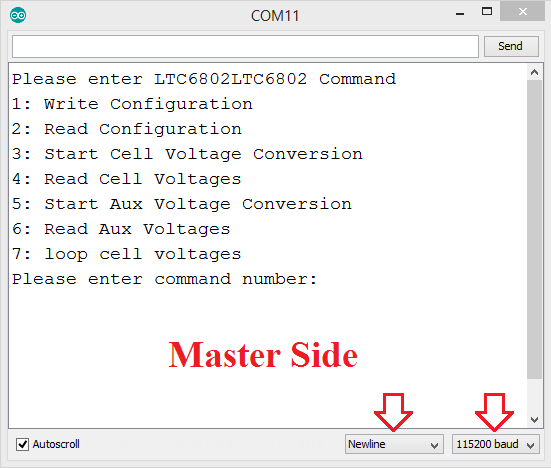
\includegraphics[width=0.45\textwidth]{figures/image15}\;
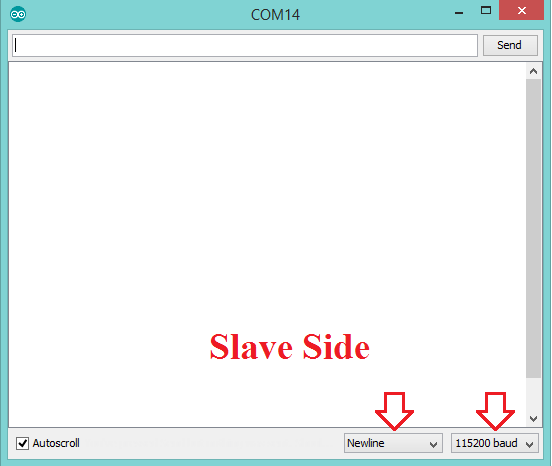
\includegraphics[width=0.45\textwidth]{figures/image16}
\caption{Selecting the baud rate for communication}
    \label{fig:serialBaud}
\end{figure}

\subsection{Step (7): Applying the Test.}
In the serial monitor of master side you can write a command number from 1 to 7 and check the received data in the serial monitor of slave side. Figure.\ref{fig:serialTest} shows what we get when we write command (1) and press ENTER key
\begin{figure}[h]
    \centering
    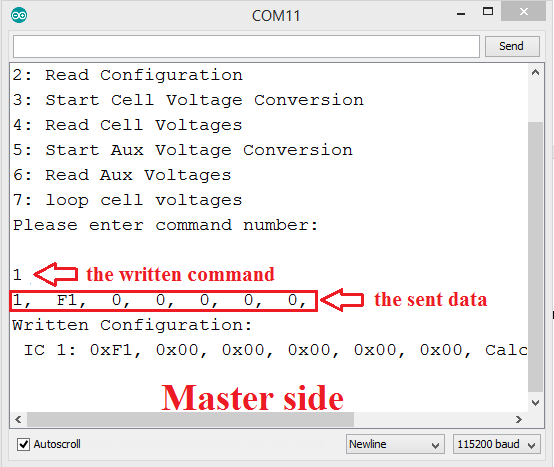
\includegraphics[width=0.45\textwidth]{figures/image17}\;
    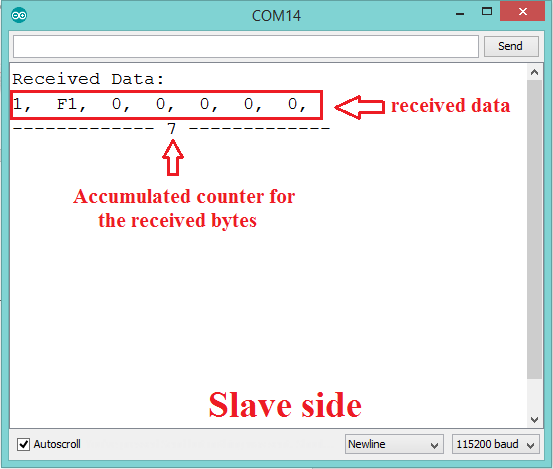
\includegraphics[width=0.45\textwidth]{figures/image18}
    \caption{Serial communication and protocol test}
        \label{fig:serialTest}
\end{figure}